\section{Object-Oriented Library Design}


\begin{frame}
\frametitle{Geometric Element Classes}

\begin{columns}
\column{.55\textwidth}
\begin{center}
\vspace{-5mm}
\includegraphics[width=.75\textwidth]{DofObjects}
\end{center}
\column{.45\textwidth}
\begin{itemize}
\item Abstract interface gives mesh topology
\item Concrete instantiations of mesh geometry
\item Hides element type from most applications
\item Runtime polymorphism allows mixed element types, dimensions
\item Base class data arrays allow more optimization, inlining
\end{itemize}

\end{columns}

\end{frame}


%%%%%%%%%%%%%%%%%%%%%%%%%%%%%%%%%%%%%%%%%%%%%%%%%
\frame
{
  \frametitle{Linear Algebra}
  \begin{center}
    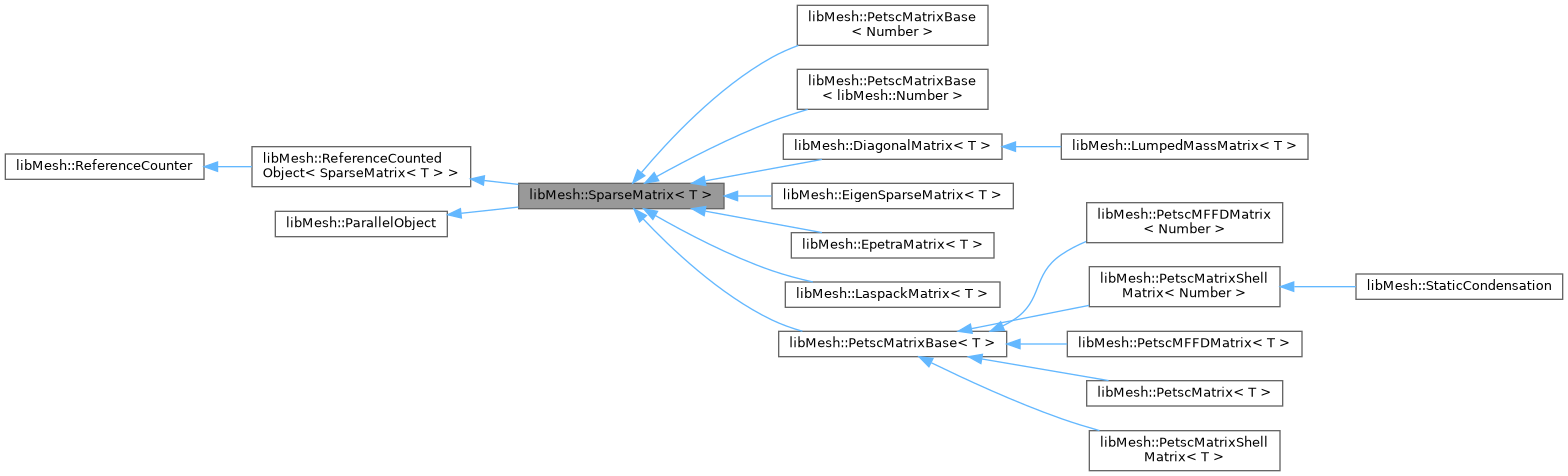
\includegraphics[width=\textwidth,trim=7.56in 0 0 0,clip]{classlibMesh_1_1SparseMatrix__inherit__graph}
  \end{center}
}



%%%%%%%%%%%%%%%%%%%%%%%%%%%%%%%%%%%%%%%%%%%%%%%%%
\frame
{
  \frametitle{I/O formats}
  \begin{center}
    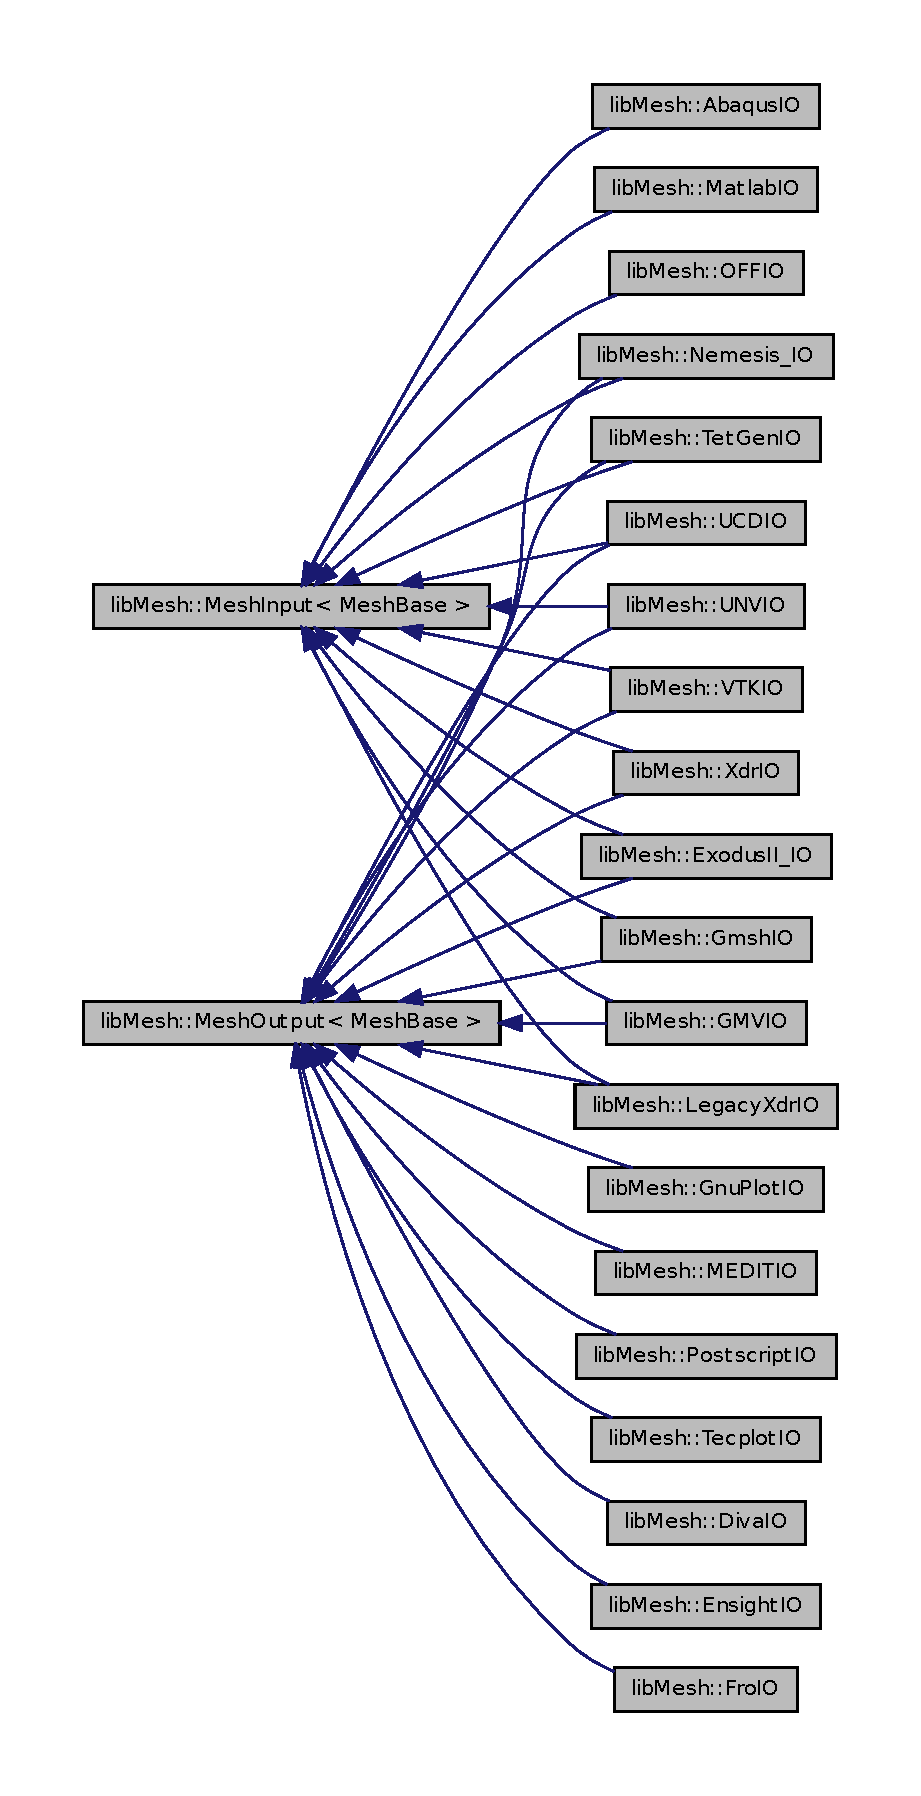
\includegraphics[height=0.9\textheight]{mesh_io}
  \end{center}
}


%%%%%%%%%%%%%%%%%%%%%%%%%%%%%%%%%%%%%%%%%%%%%%%%%
\frame
{
  \frametitle{Domain Partitioning}
  \begin{center}
    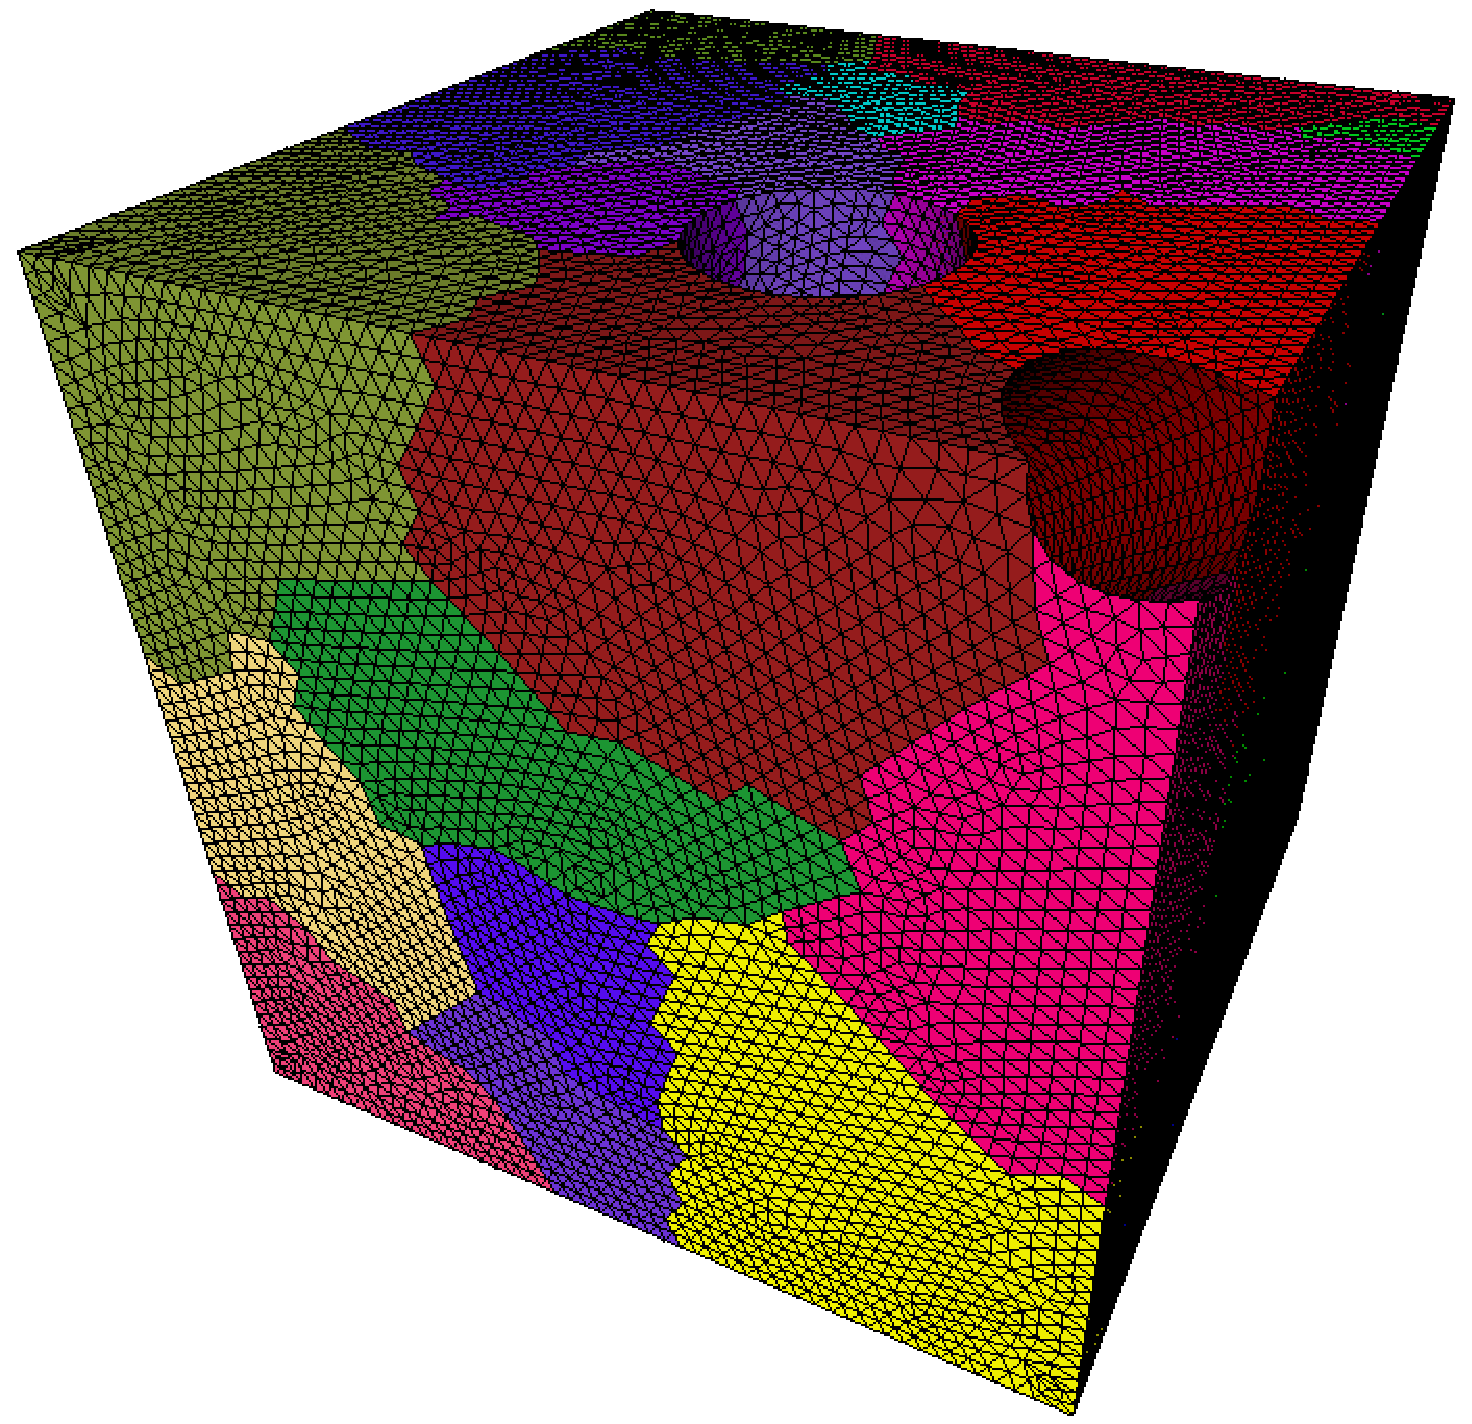
\includegraphics[width=.3\textwidth]{part_trans}
    %\\
    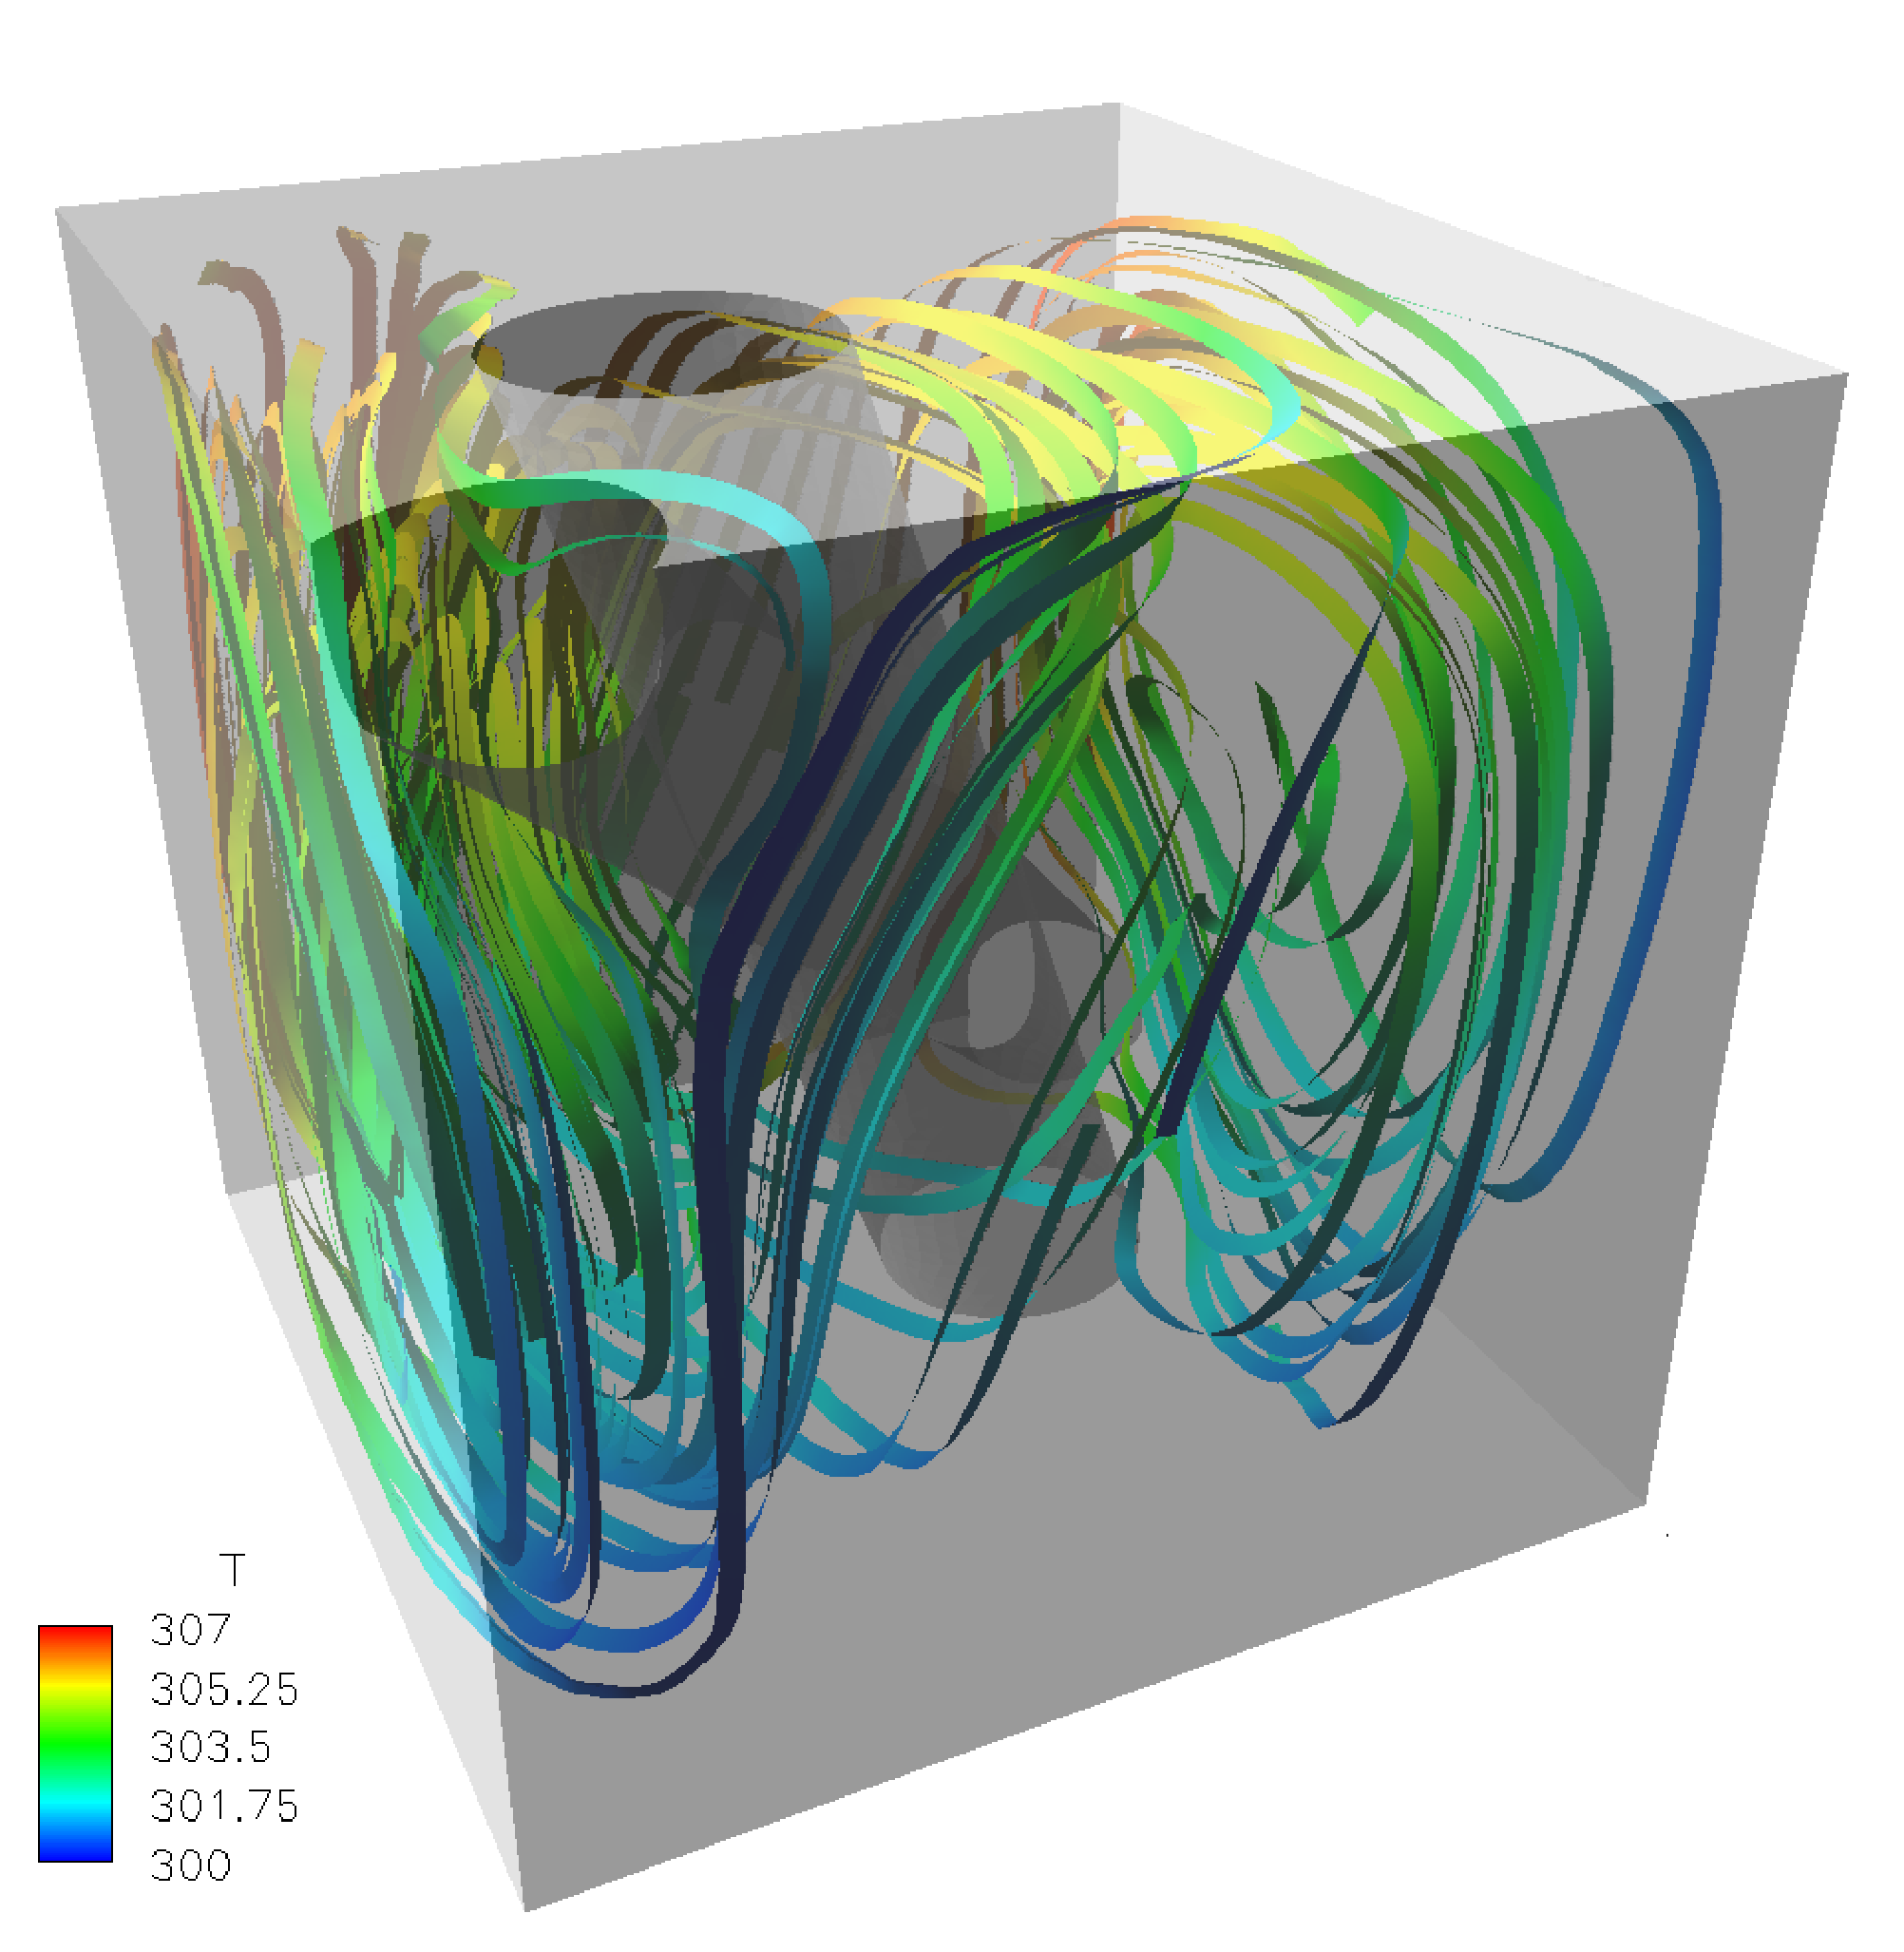
\includegraphics[width=.3\textwidth]{streamtraces}
  \end{center}  

  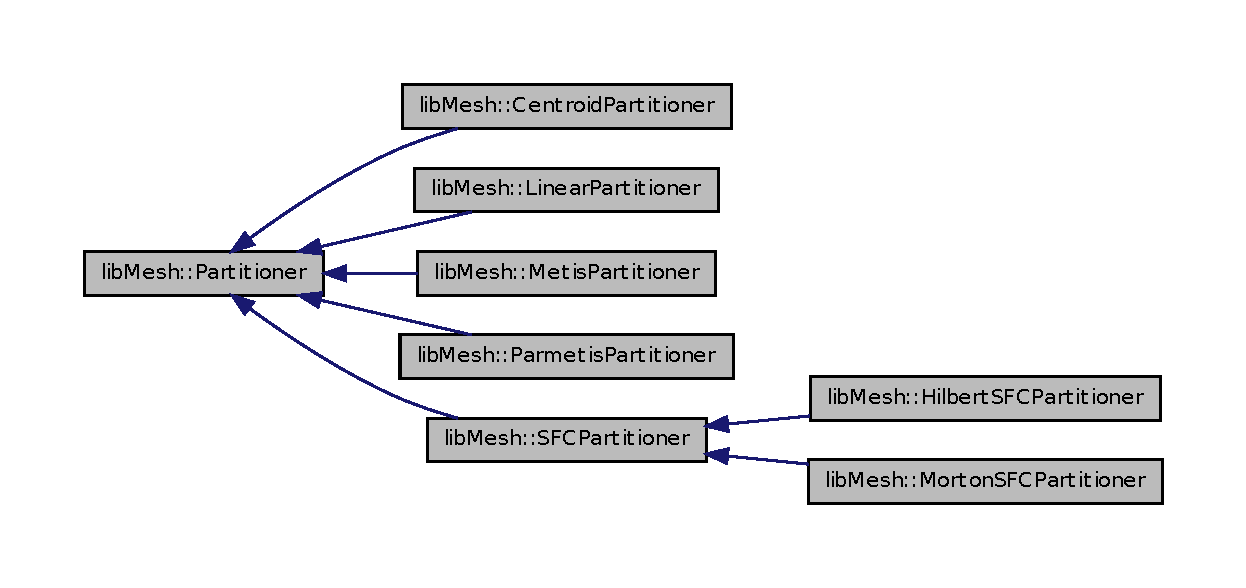
\includegraphics[width=.65\textwidth]{partitioner}
}


%%%%%%%%%%%%%%%%%%%%%%%%%%%%%%%%%%%%%%%%%%%%%%%%%
\begin{frame}
\frametitle{Mesh Data Structures}
\begin{columns}
\column{.6\textwidth}
\begin{center}
\includegraphics[width=.95\textwidth]{MeshUML}
\end{center}
\column{.4\textwidth}
%\begin{block}{}
\begin{itemize}
\item \texttt{MeshBase} gives node or element iterators, all vs active, global vs local
\item \texttt{ReplicatedMesh} or \texttt{DistributedMesh} manages synchronized or distributed data
\end{itemize}

\includegraphics[width=.75\textwidth]{ParallelMesh3}
%\end{block}
\end{columns}

\end{frame}



%%%%%%%%%%%%%%%%%%%%%%%%%%%%%%%%%%%%%%%%%%%%%%%%%
\frame
{
  \frametitle{Discretization: Finite Elements}
  \begin{center}
    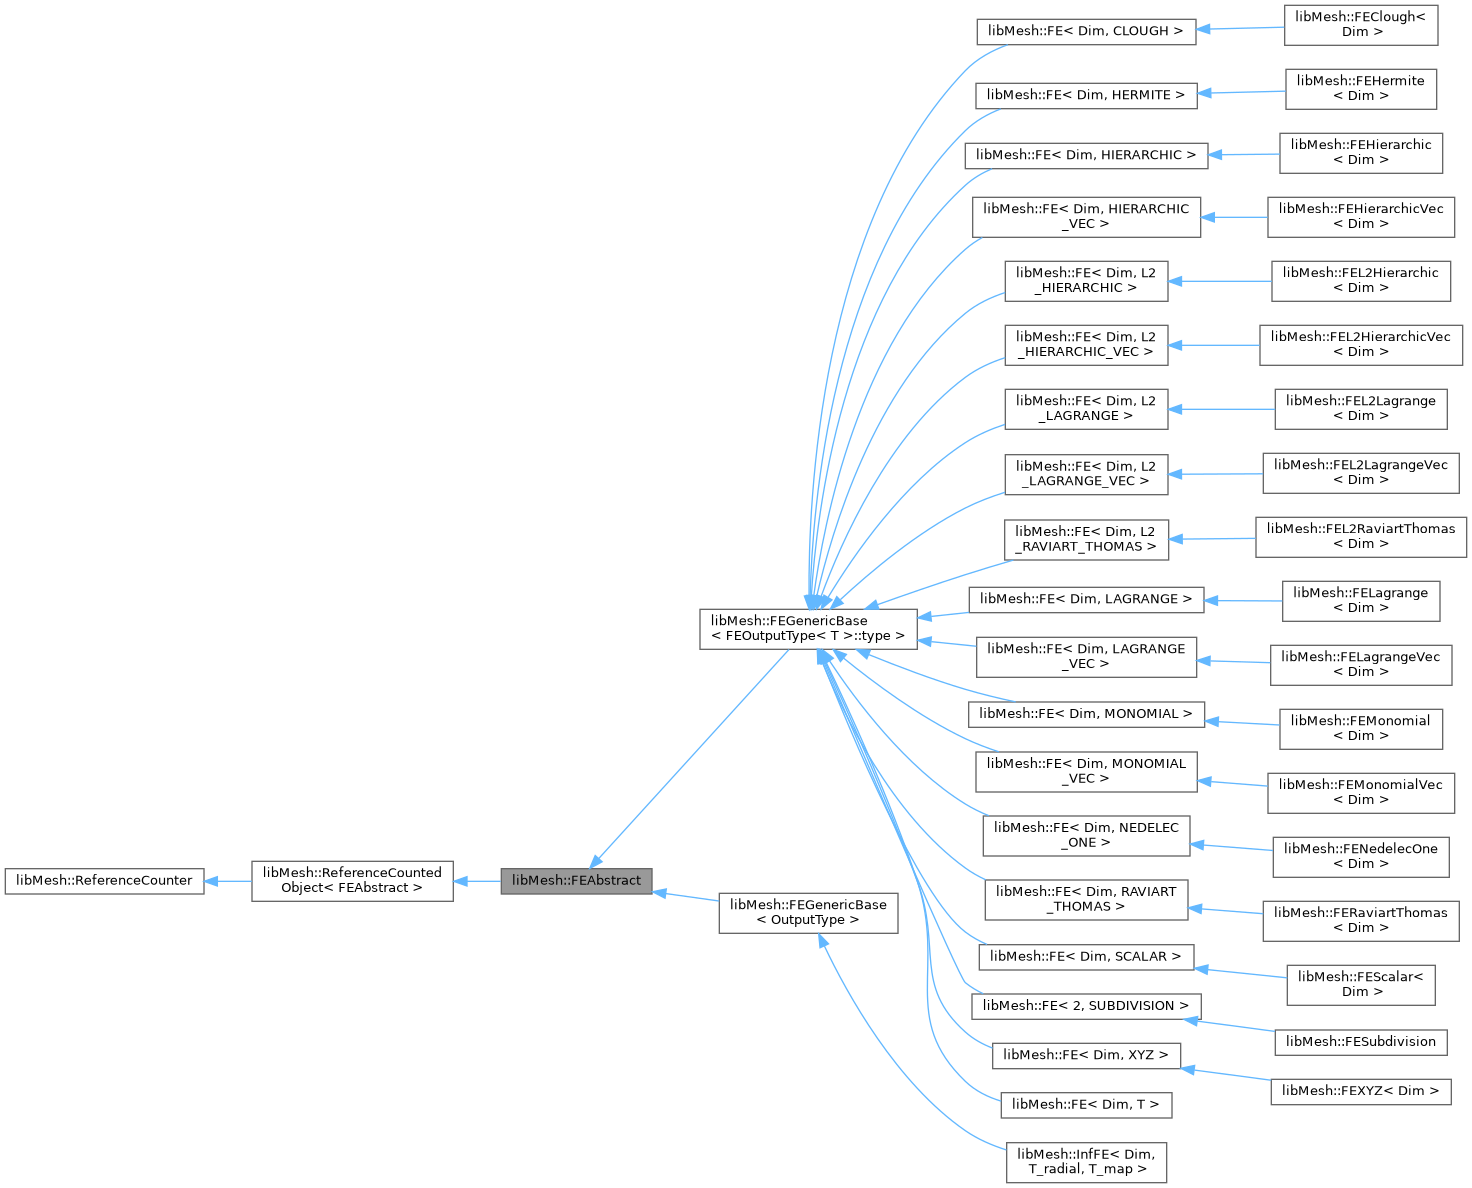
\includegraphics[width=0.9\textwidth,trim=7.4in 0 0 0,clip]{classlibMesh_1_1FEAbstract__inherit__graph}
  \end{center}
}      



%%%%%%%%%%%%%%%%%%%%%%%%%%%%%%%%%%%%%%%%%%%%%%%%%
\frame
{
  \frametitle{Algorithms: Error Estimation}
  \begin{center}
    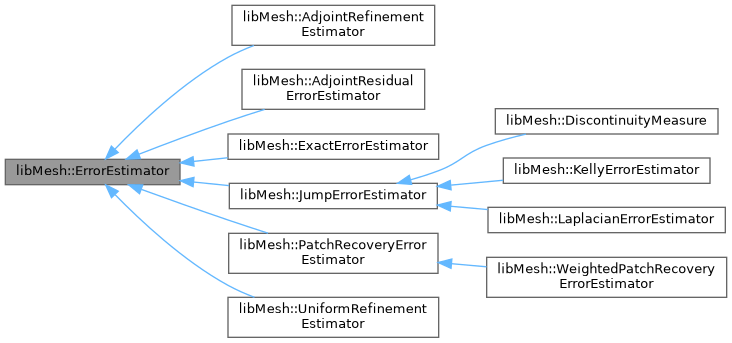
\includegraphics[width=\textwidth]{classlibMesh_1_1ErrorEstimator__inherit__graph}
  \end{center}
}


